\documentclass[../main.tex]{subfiles}

\begin{document}


\subsection{General description}

The simulation methodology is based on the work presented in\citep{gnanSilicoSynthesisMicrogel2017} and\citep{sorichettiStructureElasticityModel2023}, with the objective of create a representative polymer structure of a microgel and characterize the mechanical response under shear deformation.
This methodology creates the structure by using a mixture of two types of patchy particles.
The patchy particles are spheres of identical size and mass decorated by patches to represent interaction sites.
One type represent a \textit{Crosslinker} and is define by 1 central particle with 4 patches placed at the vertices of a circumscribed tetrahedron. %in the center particle.
The other one represent a \textit{Monomer} define by 1 central particle and 2 patches placed at the poles.\marginpar{
%Before proceeding further, it is important to mention that from now on we are going to refer to the center particle of the Crosslinker as ``CL'' and the patches as ``PA'', naturally, the center particle of the Monomer patchy particle as ``MO'' and the patches as ``PB''.
\begin{itemize}
    \item $\vec{r}_i$: Position of Crosslinker central particle
    \item $\vec{r}_j$: Position of Monomer central particle
    \item $\{\vec{r}_{\mu}^i\}$ Set of positions of the patches in the crosslinker patchy particle
    \item $\{\vec{r}_{\upsilon}^j\}$ Set of positions of the patches in the monomer patchy particle
\end{itemize}
}

The interaction between the central particles is modeled with a Weeks-Chandler-Andersen repulsive potential,
\begin{gather}
    U_{WCA}(r_{i,j}) =\left\{ 
        \begin{array}{ll}
            4\epsilon_{i,j}\left[\qty(\frac{\sigma}{r_{i,j}})^{12}-\qty(\frac{\sigma}{r_{i,j}})^6\right]+\epsilon_{i,j}, & r_{i,j}\in[0,2^{1/6}\sigma], \\
            0, & r_{i,j}>2^{1/6}\sigma
        \end{array}
\right.
    ,\label{eqn:CL-MO_interaction}
\end{gather}
where $r_{i,j}$ is the distance between the center of the central particles, $\sigma$ is the diameter of the particles and $\epsilon_{i,j}$ is the energy of the interacton.
The patch-patch interaction is modeled with an attractive potential,
\begin{gather}
    U_{\mathrm{patchy}}\qty(r_{\mu\upsilon}) = \left\{
        \begin{array}{ll}
            2\epsilon_{\mu\upsilon}\left(\frac{\sigma_p^4}{2 r_{\mu\upsilon}^4}-1\right)\exp\left[\frac{\sigma_p}{\qty(r_{\mu\upsilon}-r_{c})}+2\right], & r_{\mu\upsilon}\in\qty[0,r_c], \\
            0, & r_{\mu,\upsilon}>r_c,
        \end{array}
            \right.\label{eqn:patch-patch_interaction}
\end{gather}
where $r_{\mu\upsilon}$ is the distance between two patches, $\sigma_p$ is the diameter of the patches, $r_c$ is the cut distance of interaction set to $1.5\sigma_p$ and $\epsilon_{\mu,\upsilon}$ is the interaction energy between the patches.
Moreover, the interaction between patches is complemented by a three-body repulsive potential, defined in terms of~\eqref{eqn:patch-patch_interaction}, that provides an efficient bond-swapping mechanism making possible to easily equilibrate the system at extremely low temperatures, while at the same time, reataining the single-bond-per-patch condition\citep{sciortinoThreebodyPotentialSimulating2017},
\begin{gather}
    U_{\mathrm{swap}}(r_{l,m},r_{l,n}) = w\sum_{l,m,n}\epsilon_{m,n}U_3\qty(r_{l,m})U_3\qty(r_{l,n}),\quad r_{l,n}\in\qty[0,r_c],\label{eqn:swap_interaction}
\end{gather}
where
\begin{gather}
    U_{3}\qty(r) = \left\{
        \begin{array}{ll}
            1 & r\in\qty[0,r_{\min}], \\
            -U_{\mathrm{patchy}}\qty(r)/\epsilon_{m,n}, & r\in\qty[r_{\min},r_c]
        \end{array}
        \right.\label{eqn:swapmod_interaction}.
\end{gather}
The sum in~\eqref{eqn:swap_interaction} runs over all triples of bonded patches (patch $l$ bonded both with $m$ and $n$).
$r_{l,m}$ and $r_{l,n}$ are the distances between the reference patch and the other two patches.
The parameter $\epsilon_{m,n}$ is the energy of repulsion and $w$ is used to tuned the swapping ($w=1$) and non-swapping bonds ($w\gg1$). 
The cut off distance $r_c$ is the same as in the potential of interaction between patches, meanwhile the minimum distance $r_{\min}$ is the distance at the minimum of~\eqref{eqn:patch-patch_interaction}, \textit{i.e.} $\epsilon_{m,n}\equiv\abs{U_{\mathrm{patchy}}(r_{\min})}$.
Finally, the energy of interaction between crosslinker patches ($\epsilon_{\mu^i,\mu^i}$) are set to $0$ to allow only crosslinker-monomer and monomer-monomer bonding (figure~\ref{fig:intento2}).

\begin{figure}[ht]
    \centering 
    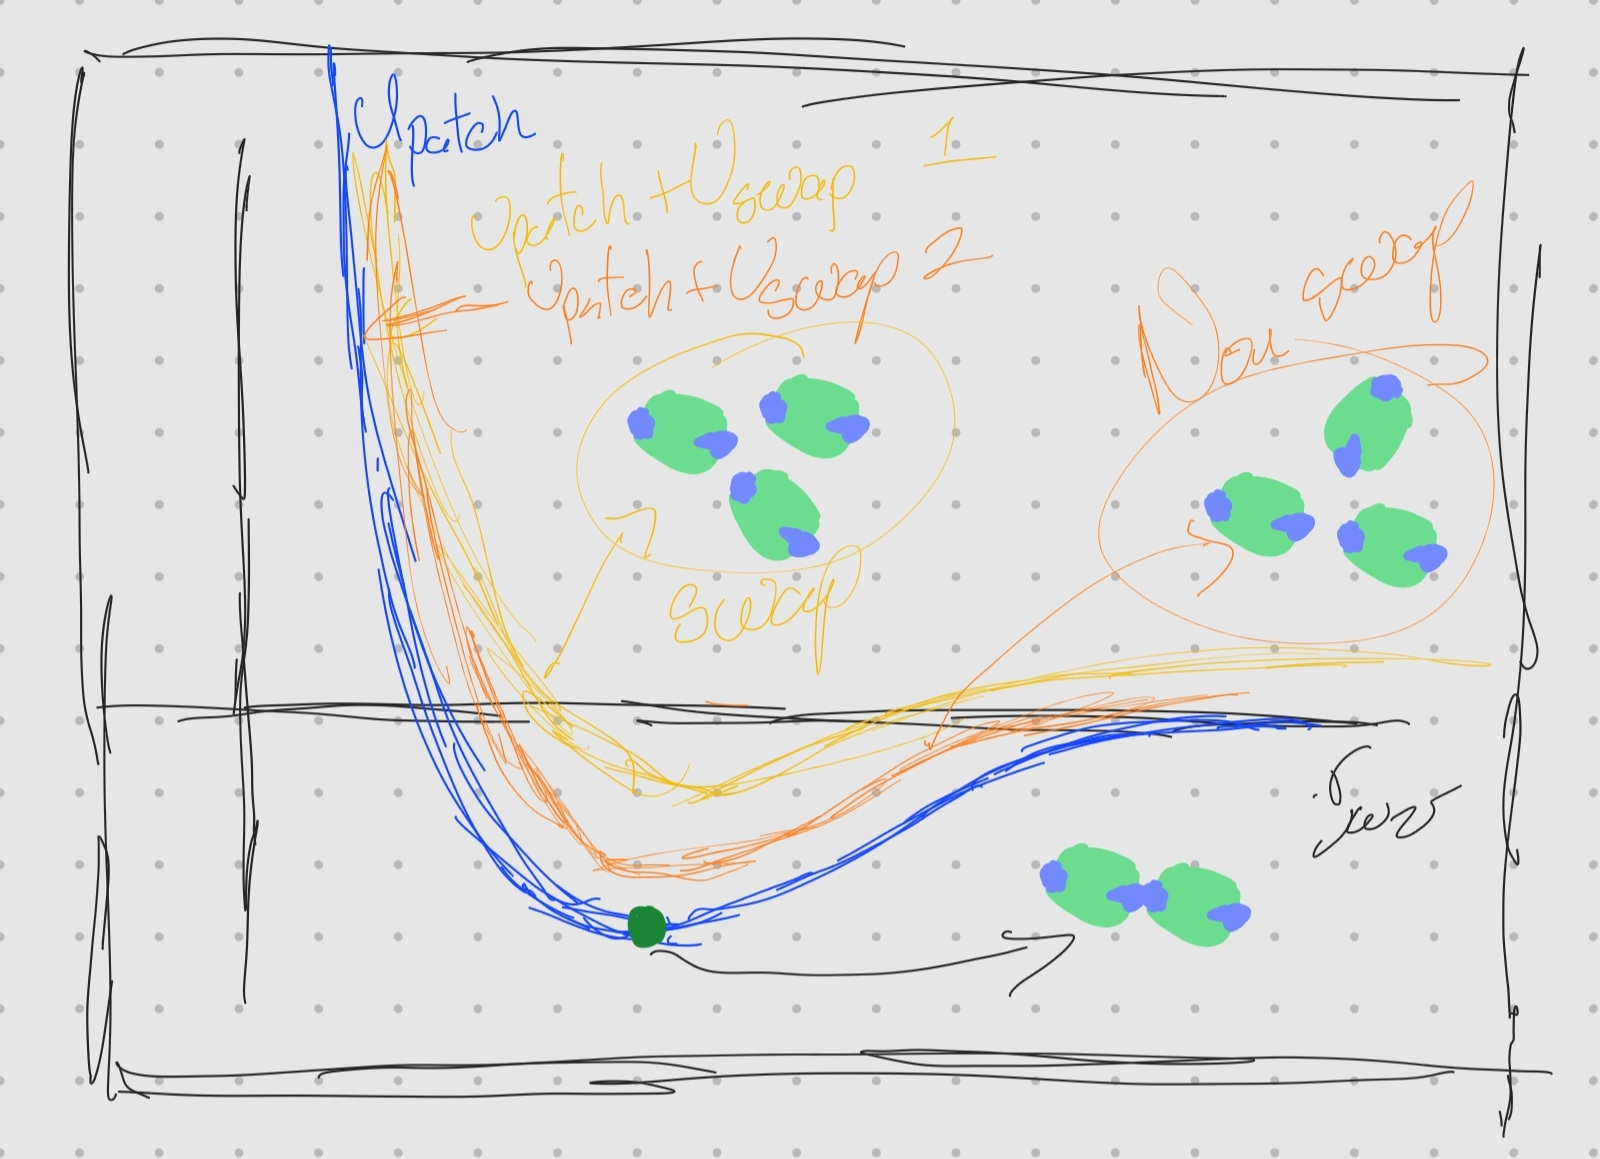
\includegraphics[width=0.8\textwidth]{../../imgs/potentia-interactions.jpg}
    \caption{La idea de la figura es poner el pontecial de interacción entre paches y ver el efecto del pontecial de 3 cuerpos cuando $w=1$ y cuando $w\gg1$.}\label{fig:intento}
\end{figure}


\begin{figure}[ht]
    \centering 
    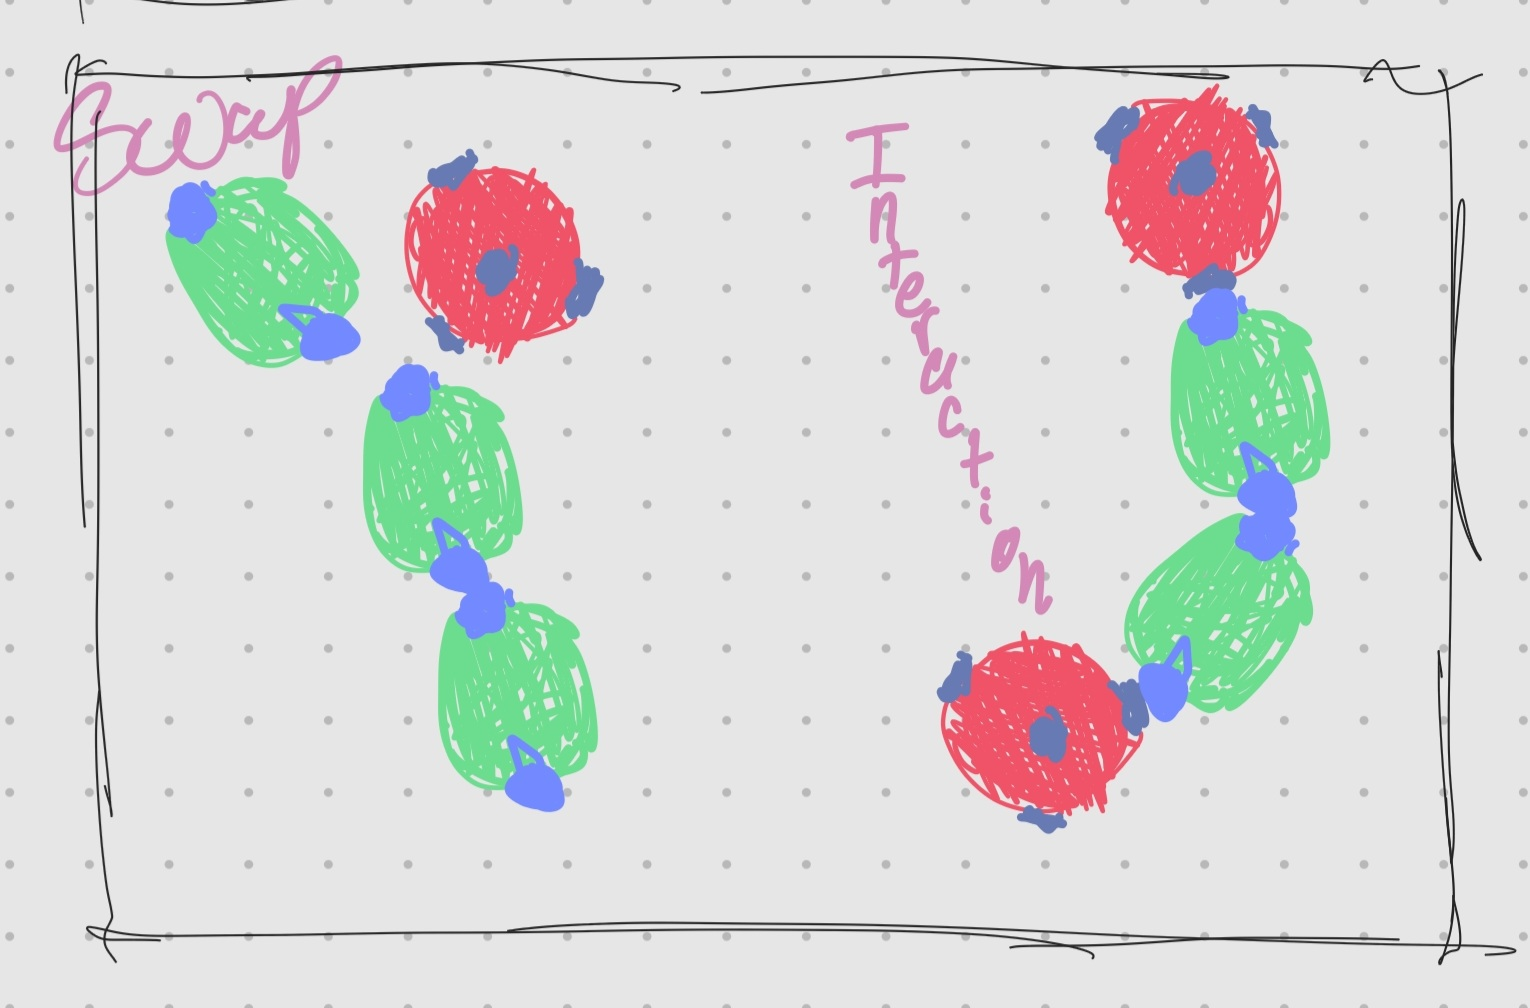
\includegraphics[width=0.8\textwidth]{../../imgs/patches-interaction.jpg}
    \caption{La idea de esta es mostrar las posibles configuraciones (monomero-monomero, monomero-crosslinker y un poco de pontecial de 3 cuerpos)}\label{fig:intento2}
\end{figure}



%Once we defined the interactions between the particles in the system, we define a simulation protocol divided in the following processes, assembly and shear.
%Which are going to be described in detail in the following sections.


%After the assembly process, the structure is analyse to see if the structure percolate or not and verify if there are only binary patch-interactions, otherwise we checked the implementation of the potentials or the parameters.
%Once the hydro-gel structure meet the requirements we start with the shear process and monitored the temperature and energy to see if the simulaiton was converging.
%Once those tests done, the mechanical response was analyze thru the components of the stress tensor and structure characterization.

\subsection{Assembly of the network}

We perform molecular dynamics (MD) simulations at fixed temperature $T = kBT/\epsilon = 0.05$, where kB is the Boltzmann constant. 
Thanks to such a low temperature, the system tends to maximize the number of bonds. 
In addition, owing to the bondswapping mechanism, the system is able to continuously restructure itself, until the large majority of possible bonds are formed.
It is important to said that the main difference between the articles cited and the implementation in this htesis are the absence of FENE bonds and the swelling potential.

%because part of the exploration is to analyze what happen in the deformation if the interactions between crosslinker and monomer can swap.


\begin{comment}
\subsection{LAMMPS implementation}

We use reduce units, Lennard-Jones units.

To create the patchy particles, the \verb|zero| bond style is used.
The reason to use this, is because bond forces and energies are not computed, but the geometry of bond pairs is accessible to other commands (\href{https://docs.lammps.org/bond_zero.html}{Ref}).

The pair styles used in the simulation are: \verb|hybrid/overlay|, \verb|zero|, \verb|lj/cut|, \verb|table| and \verb|threebody/table|.
The \verb|hybrid/overlay| style is used because superimposed multiple potentials in an additive fashion (\href{https://docs.lammps.org/pair_hybrid.html}{Ref}).
The rest of pair styles are to implement the potentials described in \ref{subsec:Potentials}.

The length of the box is set, such that the desire Monomers and Cross-Linkers can be spawn.
The mass of the patches are set to be the half mass of the CL and MO.

The \verb|pair_coeff| commands where set to accomplish the simulation describe in \ref{sec:descriptionSimulation}.
With respect the \verb|create_atoms| command, the \textit{overlap} keyword was assign to a value of the diameter of CL and MO.

Then, the \verb|rigid/small| fix command is used to create the Monomers and Cross-Linkers particles.
This is because, this command is typucally best for a system with large number of small rigid bodies\href{https://docs.lammps.org/fix_rigid.html}{Ref}.

The \verb|neighbor| command was set of type bin with a value of 1.8 and the \verb|neigh_modify| command with the exclude keyword was added to save needless computation due to the rigid bodies (\href{https://docs.lammps.org/neigh_modify.html}{Ref}).

Then, a Langevin thermostat is used with a velocity-Verlet time integration algorithm to perform Brownian dynamics with the commands \verb|fix lagevin| and \verb|fix nve|.
The Langevin thermostat is implemented to models an interaction with a background implicit solvent, in this case water.
Meanwhile, the \verb|fix nve| help to create a system trajectory consistent with the microcanonical ensemble, in which the number of particles, volume and energy remains constant.

finally, multiple \verb|computes| are used to get the potential, kinetic and total energies, temperature and voronoi analysis.

\subsection{Packing fraction}

To approximate a desire packing fraction in the simulation we consider that the packing fraction represent the ratio between the volume of the particle with respect the total volume of the simulation box,
\begin{gather*}
    \phi = \frac{V_{\mathrm{particles}}}{V_\mathrm{box}}.
\end{gather*}
Since, the packing fraction and the volume of the particles are defined, we compute for the volume of the simulation box, and then assume that the simulation box is a cube.

We use a ``ghost'' particle to compute the approximate volume, due to easier calcalculations.
We assume a sphere of $r_{\mathrm{CP}}+r_{\mathrm{patch}}$ and compute the volume of that ``ghost'' sphere.
\begin{gather*}
    V_{\mathrm{ghost}} = \frac{3}{4}\pi (r_{\mathrm{CP}}+r_{\mathrm{patch}})^{3}
\end{gather*}
considering that $r_{\mathrm{CP}}=0.5, r_{\mathrm{patch}}=0.2$, the volume is,
\begin{align*}
    V_{\mathrm{ghost}} &= \frac{3}{4}\pi (0.7)^{3} \\
                       &= 0.8.
\end{align*}

Now, to compute the dimensions of the simulation box,
\begin{align*}
    V_\mathrm{box} &= \frac{V_{\mathrm{particles}}}{\phi} \\
                   &= \frac{0.8}{\phi} \\
    \frac{V_\mathrm{box}}{3}&= \frac{1}{3}\frac{0.8}{\phi} \\
    L &= \frac{0.8}{3\phi}
\end{align*}

\end{comment}

\end{document}
